\documentclass[12pt,a4paper]{article}
\usepackage[utf8]{inputenc}
\usepackage[warn]{mathtext}
\usepackage[english,russian]{babel}
\usepackage{indentfirst}
\usepackage{misccorr}
\usepackage[warn]{mathtext}
\usepackage{subcaption}
\captionsetup{compatibility=false}
\usepackage{graphicx}
\usepackage{wrapfig}
\usepackage{amsmath}
\usepackage{floatflt}
\usepackage{float}
\usepackage{amssymb}
\usepackage{color}
\usepackage{lscape}
\usepackage{hvfloat}
\usepackage{amsfonts}
\usepackage{euscript}
\usepackage{mathtext}
\graphicspath{{pictures/}}
\DeclareGraphicsExtensions{.png,.jpg, .jpeg}
\usepackage[left=20mm, top=18mm, right=20mm, bottom=18mm, footskip=10mm]{geometry}
\linespread{1}



\begin{document} 
\begin{titlepage}
  \begin{center}
    \large
    Московский Физико-Технический Институт
    
    (Национальный исследовательский университет)
    \vspace{0.5cm}

   
    \vspace{0.25cm}
 
    \vfill
 
    \vfill

    \textsc{\bf{Лабораторная работа}}\\[5mm]
    
    {\LARGE  Автоэлектронная эмиссия}
  \bigskip
    \vfill
    
\end{center}
\vfill
\begin{flushright}


    \textbf{Выполнили} студенты группы Б04-005 \\
    Назарова Анна Сергеевна\\
    Спирандэ Екатерина Константиновна\\
    Юн Максим Игоревич\\
    Ярышева Ирина Михайловна\\

\end{flushright}

\bigskip

\vfill

\begin{center}
  Долгопрудный, 2022 г.
\end{center}
\end{titlepage}



\section*{Аннотация}
В данной работе проводятся исследования автоэмиссионных свойств вольфрамового острия и катодов, изготовленных из углеродных волокон. Исследуются механизмы нестабильности автоэмиссионного тока на примере углеродных трубок.\\

\noindent\textbf{Цель работы: }исследование автоэмиссионных свойств и механизмов нестабильности автоэмиссионного тока на примере катода, изготовленного из углеродных волокон. Получение ВАХ с помощью электронного осциллографа.
\\ 
\noindent\textbf{Оборудование: }источник напряжения, стрелочный амперметр, вольтметр, электронный осциллограф, резистор, игла из вольфрама, катод из углеродных трубок.

\section{Теоретическая часть}
\subsection{Автоэлектронная эмиссия металлов}

При наличии электрического поля над поверхностью металла наблюдается внешняя автоэлектронная эмиссия (автоэмиссия, холодная эмиссия, туннельная эмиссия). \textbf{Автоэлектронная эмиссия} - явление испускания электронов в вакуум с поверхности твердого тела или другой среды под действием очень сильного электрического поля напряженностью $10^{7}-10^{8}$ В/см.

Автоэлектронная эмиссия является эмиссией, не требующей возбуждения электронов. Суть явления состоит в туннелировании электронов сквозь потенциальный барьер на поверхности тела. Такое туннелирование становится возможным за счет искривления потенциального барьера при приложении внешнего поля. При этом появляется область пространства вне тела, в которой электрон может существовать с той же полной энергией, которой он обладает, находясь в теле. Таким образом, автоэлектронная эмиссия обусловлена волновыми свойствами электронов.

Впервые такое объяснение автоэмиссии было предложено в 1928 году Фаулером и Нордгеймом. Ими впервые была получена формула, описывающая взаимосвязь плотности автоэлектронного тока $j$ с напряженностью электрического поля $E$:
\begin{equation}
    j = \frac{e^3}{4\pi^2\hbar}\frac{E_f^{1/2}}{W_a\varphi^{1/2}} E^2 \exp(-\frac{4}{3e}\frac{\sqrt{2m}}{\hbar}\cdot\frac{\varphi^{3/2}}{E}),
\end{equation}
%\begin{figure}[H]
%\centering
%	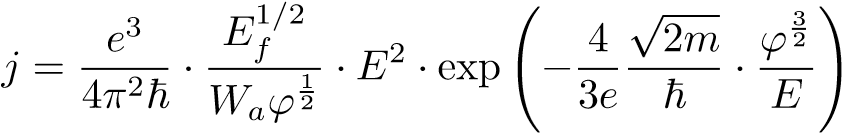
\includegraphics[width=0.5\linewidth]{Form1.png}
%\end{figure}

где $\varphi = W_{a} - E_{f}$ – работа выхода, $E_{f}$ – энергия Ферми, $W_{a}$ – уровень вакуума (все энергии отсчитываются от дна зоны проводимости).

Эта формула получена для полубесконечного металла с плоской поверхностью, подчиняющегося модели Зоммерфельда и находящегося при температуре $T = 0 K$.
При выводе этой формулы Фаулер и Нордгейм предположили, что потенциальный барьер на поверхности тела имеет вид, показанный на  рис.1 (кривые $A$ и $B$):

\begin{figure}[h]
\centering
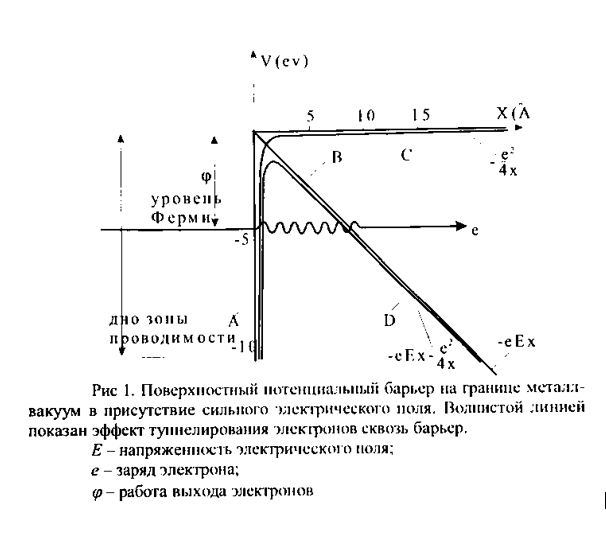
\includegraphics[width=12cm]{Pic1.png}
\end{figure}

Позднее в 1929 году Нордгейм предложил ввести в рассмотрение силы электростатического изображения рис.1 (кривые $C$ и $D$). Это привело к выражению:
\begin{equation}
    j = A\frac{E^2}{\varphi}\exp{B\frac{\varphi^{3/2}}{E}\theta(y)},
\end{equation}
%\begin{figure}[H]
%\centering
%	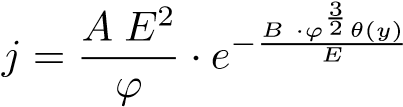
\includegraphics[width=0.2\linewidth]{Form2.png}
%\end{figure}
где $A \equiv \frac{e^{3}}{16\pi^2\hbar}$, $B \equiv \frac{4\sqrt{2m}}{3e\hbar}$, $\theta(y)$ - спецфункция, которая была табулирована Нордгеймом, и получила название «функция Нордгейма». При не очень близких к $0$ или $1$ значениях аргумента функция Нордгейма хорошо приближается аналитическим выражением $\theta(y) = 0.965 - 0.739y^2$.

Подставив $\theta(y)$ в (2), получим:
\begin{equation}
    j = A'\frac{E^2}{\varphi}exp(-B'\frac{\varphi^{3/2}}{E}),
\end{equation}
%\begin{figure}[H]
%\centering
%	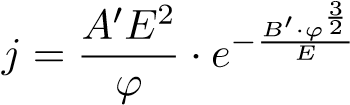
\includegraphics[width=0.2\linewidth]{Form3.png}
%\end{figure}
где $A' = \frac{e^{3}}{8 \pi h}e^{0.739\cdot\frac{\frac{8\pi}{3e}(2m\phi^{3})^{1/2}}{hE}}$, $B' \equiv 0.965\cdot\frac{\frac{8\pi}{3e}(2m\phi^{3})^{1/2}}{hE}$, $y \equiv \frac{\sqrt{e^{3}E}}{\phi}$, $\alpha$ - – угол наклона получившейся кривой.

Строго говоря, теория Фаулера-Нордгейма применима только при температуре $T = 0K$. Однако, так как незначительное увеличение температуры мало меняет распределение электронов в металле, лишь размывая его на величину порядка $kT$ вблизи уровня Ферми, то выводы теории остаются качественно верны при температурах, определяемых условием $kT \ll \varphi$. При комнатной температуре, например, $kT = 2.6 \cdot 10^{-2}$ эВ, в то время как характерное значение работы выхода $\varphi$ = 3...6 эВ.

Если построить график зависимости $\ln(\frac{j}{E^{2}})$ от $\frac{1}{E}$ , то соответствующая кривая окажется практически прямой линией в узкой области напряженности поля, которая характерна для типичного автоэмиссионного эксперимента. Эта прямая называется графиком Фаулера-Нордгейма, а соответствующие координаты - координаты Фаулера-Нордгейма ($\ln(\frac{j}{E^{2}})$, $\frac{1}{E}$).

Наклон графика выржается формулой: $$S_{FN} = \frac{d \ln{\frac{j}{E^2}}}{d \frac{1}{E}} = -0.683\cdot s(\frac{3.79 \sqrt{E}}{\varphi}) \cdot \varphi^{\frac{3}{2}}$$
где $s(y)$:
\begin{figure}[H]
\centering
	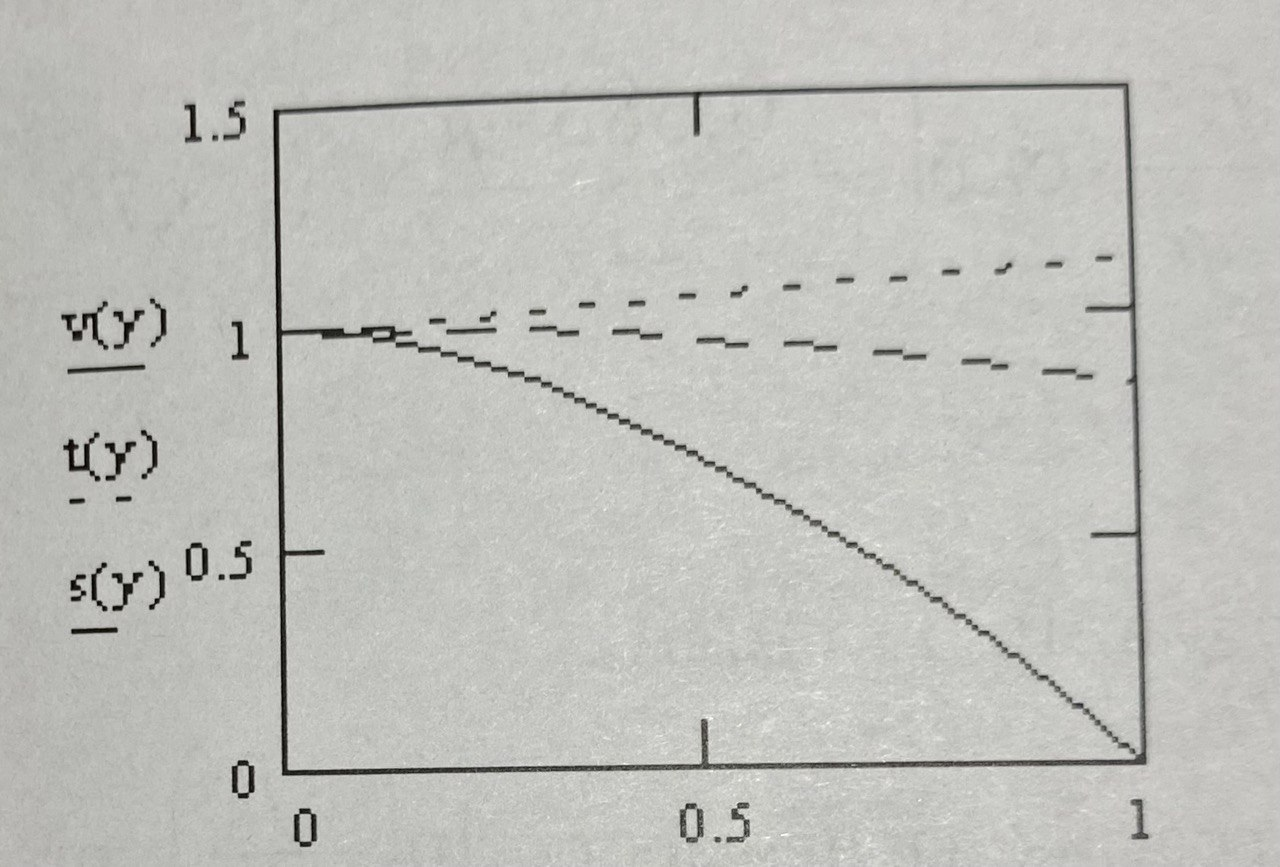
\includegraphics[width=0.3\linewidth]{ы(н).jpg}
\end{figure}
$s(y)$ в узкой области напряжённости поля можно считать константой. В рабочем диапазоне токов и напряжений, эту функцию можно приближённо считать равной 1.

\subsection{Одноэмитттерные системы}

\begin{equation}
 E = \beta U
\end{equation}
\begin{equation}
I = S_{e}j,
\end{equation}
где $S_{e}$ – площадь поверхности эмиттера, $\beta$ – форм-фактор острия.
Таким образом, если построить график зависимости $\ln(\frac{I}{U^2})$, то мы получим прямую (прямая Фаулера-Нордгейма для полного тока и напряжения), тангенс угла наклона которой будет определяться выражением:

\begin{equation}
\tan(\alpha)=-0.683\cdot s(\frac{3.79 \sqrt{\beta \cdot U}}{\phi}) \cdot \frac{\phi^{\frac{3}{2}}}{\beta}
\end{equation}
Принимая во внимание, что $s(y)$ можно считать равной 1:

\begin{equation}
\tan(\alpha) = -0.683 \cdot \frac{\varphi ^{\frac{3}{2}}}{\beta}
\end{equation}

\subsection{Многоэмитттерные системы}


Формула (7) справедлива для одноэмиттерных систем - когда имеется одно эмитирующее острие с форм-фактором $\beta$. Однако, если имеется несколько эмиссионых центров, то, пренебрегая в простейшем случае взаимным влиянием центров (экранировкой), получим выражение:

\begin{equation*}
I = \sum_i I_i
\end{equation*}


Анализ этого выражения в общем случае не представляется возможным,тем не менее для реального катода часто выполняется условие малого разброса значений форм-фактора от центра к центру. В этом случае форм-фактор каждого центра можно заменить средним значением. Имеем:

\begin{equation}
I = S \frac{A}{t^2(y_0)} \frac{\beta^2 U^2}{\phi} exp (-\beta \frac{\phi^{3/2}}{\beta U} \nu (y_0))
\end{equation}
где $y_0 = 3.79\frac{\sqrt{\beta U}}{\varphi}$, A  и B - константы

Суммарная площадь рабочей поверхности $S$ определяется выражением:

\begin{equation*}
S = N S_0 = N \alpha r^2,
\end{equation*}
где $\alpha$ - коэфицент формы эмиссионного центра, $r$ - характерный размер центра

Форм-фактор центра можно выразить формулой:

\begin{equation}
\beta = \frac{1}{kr \ln(\frac{R}{r})},
\end{equation}

\subsection{Нестабильность эмиссионого тока}
Основные причины нестабильности тока автоэлектронных катодов:
\begin{enumerate}
\item Разрушение поверхности под действием ионной бомбардировки остаточных газов: приводит к нестабильности микрогеометрии катода
\item Адсорбция и десорбция атомов остаточных газов: вызывает изменение локальной работы выхода
\item Разрушение или изменение геометрии эмиссионных центров под действием пондеромоторных нагрузок
\item Разрушение центров из-за нарушения теплового режима катода при больших плотностях тока
\end{enumerate}

В результате эксперимента получается набор точек, которые апроксимируются:

\begin{equation*}
\ln (\frac{I}{U^2}) = A - B \frac{1}{U}
\end{equation*}

Зависимость $A$ от $\ln B$ позволяет качественно определить причину нестабильности тока. 

\begin{itemize}
	\item Изменение числа эмиссионных центров: $A$ - изменяется, $\ln B$ - постоянный
	\item Изменение работы выхода: $A$ - линейно зависит от $\ln B$ с работой выхода $1.5$
	\item Изменение размеров центра: $A+2 \ln B$ - линейно от $\exp(-\frac{A}{2})$
\end{itemize}

% subsection нестабильность_эмиссионого_тока (end)

\section{Техника автоэлектронной микроскопии} % (fold)
\label{sec:техника_автоэлектронной_микроскопии}

\subsection{Констpукция прибора} % (fold)
\label{sub:констуркция_прибора}
Для получения автоэмиссионного тока необходимо приложить к поверхности образца сильное электрическое поле. Проще всего это сделать на поверхноcти с большой кривизной. На прозрачное покрытие, служающее анодом, подается высокое положительное напряжение, объект исследования - острие крепится в специальной трубке.

Электроны, эмитированные с острия, ускоряются приложенным напряжением и, попадая на люминофор, вызывают его свечение. Создаются автоэлектронное изображение эмиттирующей поверхности.
% subsection констуркция_прибора (end)

\subsection{Увеличение и разрешение автоэлектронного микроскопа} % (fold)
\label{sub:увелечение_и_разрешение_автоэлектронного_микроскопа}

Эмиттированные электроны покидают острие практически перпендикулярно его поверхности, поэтому увелечение микроскопа может быть записано в виде:

\begin{equation*}
	M = \frac{R}{\gamma^2 r},
\end{equation*}
где $R$ - растояние эмиттер-экран, $\gamma$ - фактор сжатия (обычно $1.5-1.9$), $r$ - радиус острия.

Разрешение микроскопа выражается следующим образом:

\begin{equation*}
\delta = C_1 \sqrt{r} \sqrt{(\frac{C_2}{\sqrt{V}}+ \frac{C_3}{\sqrt{\phi}})}
\end{equation*}

% subsection увелечение_и_разрешение_автоэлектронного_микроскопа (end)

\subsection{Углеродные материалы и катоды на их основе} % (fold)
\label{sub:углеродные_материалы_и_катоды_на_их_основе}

Среди известных углеродных материалов наиболее полходящим для создания катода является графит и полиакрилонитрильные углеродные волокна. 

Слои атомов углерода такого волокна образуют фибриллы, которые в зависимости от условий и температуры нагрева в процессе получения имеют размер по большой оси $1000$ нм, и диаметр $50$ нм. Фибриллы связаны между собой аморфными областями. Такая связь обеспечивает эластичность углеродных волокон. Эмиссионными центрами у такого вида катода являются многочисленные микровыступы, образованные выходящими на торцевую поверхность волокна фибриллами. Катод такой структуры обладает высокой стабильностью тока и большим сроком службы.

Однако, в ходе работы с катодами на основе волокон было установлено, что у автоэмиссионного катода, состоящего из пучка углеродных волокон, происходит отклонение периферийных волокон под действием электростатических сил. Для уменьшения влияния этого эффекта пучки вытравливают спцеаильным образом, придавая им оптимальную форму.

\section{Экспериментальная установка}

Экспериментальная часть исследования автоэмиссионных свойств вольфрамового острия проводится с вакуумным стендом, где внутри вакуумной камеры размещен исследуемый образец. Схематическая блок-схема представлена на рис. \ref{ust}

\begin{figure}[H]
	\centering
	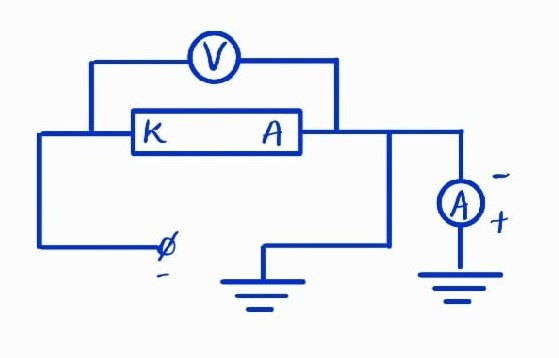
\includegraphics[scale=0.4]{sheme.jpg}
	\caption{Блок-схема установки}
	\label{ust}
\end{figure}

В нашей работе исследуются автоэмиссионные свойства и механизмы нестабильности автоэмиссионного тока на примере катодов, изготовленных из углеродных волокон. Исследуемые автокатоды находятся в отпаянной стеклянной лампе, схема которой представлена на рис. \ref{pic2}

\begin{figure}[H]
	\centering
	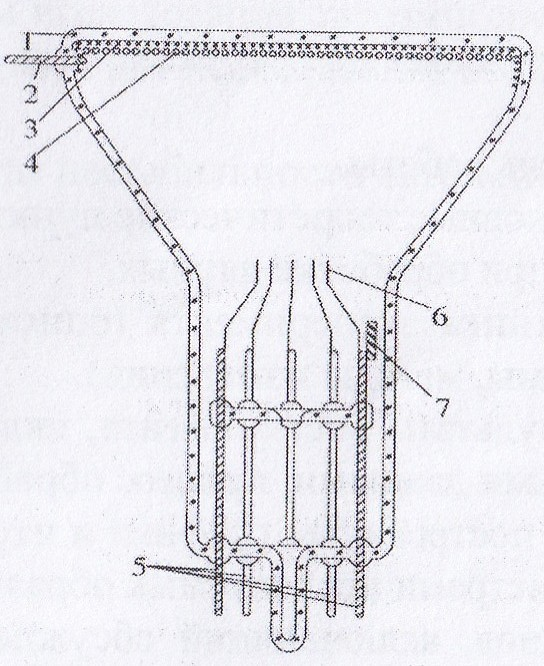
\includegraphics[width=110pt]{ust.jpg}
	\caption{Конструкция автоэмиссионной лампы на основе углеродных волокон, для исследования автоэмиссионных свойств углеродных волокон}
	\label{pic2}
\end{figure}

\section{Практическая часть}

\subsection{Исследование автоэмиссионных свойств вольфрамового острия}
Снимем вольт-амперную характеристику катода. В качестве катода выступает очищенное вольфрамовое острие. На основании полученных данных построим график зависимости $I = f(U)$.\\
\textbf{Таблица 1. }Данные для построения вольт-амперной характеристики вольфрамового острия
\begin{table}[h!]
\begin{tabular}{|l|l|l|l|l|}
\hline
$I$, мкА & 1,5  & 2,1  & 3    & 3,75 \\ \hline
$U$, В   & 1996 & 2328 & 2892 & 2914 \\ \hline
\end{tabular}
\end{table}
\begin{figure}[H]
\centering
	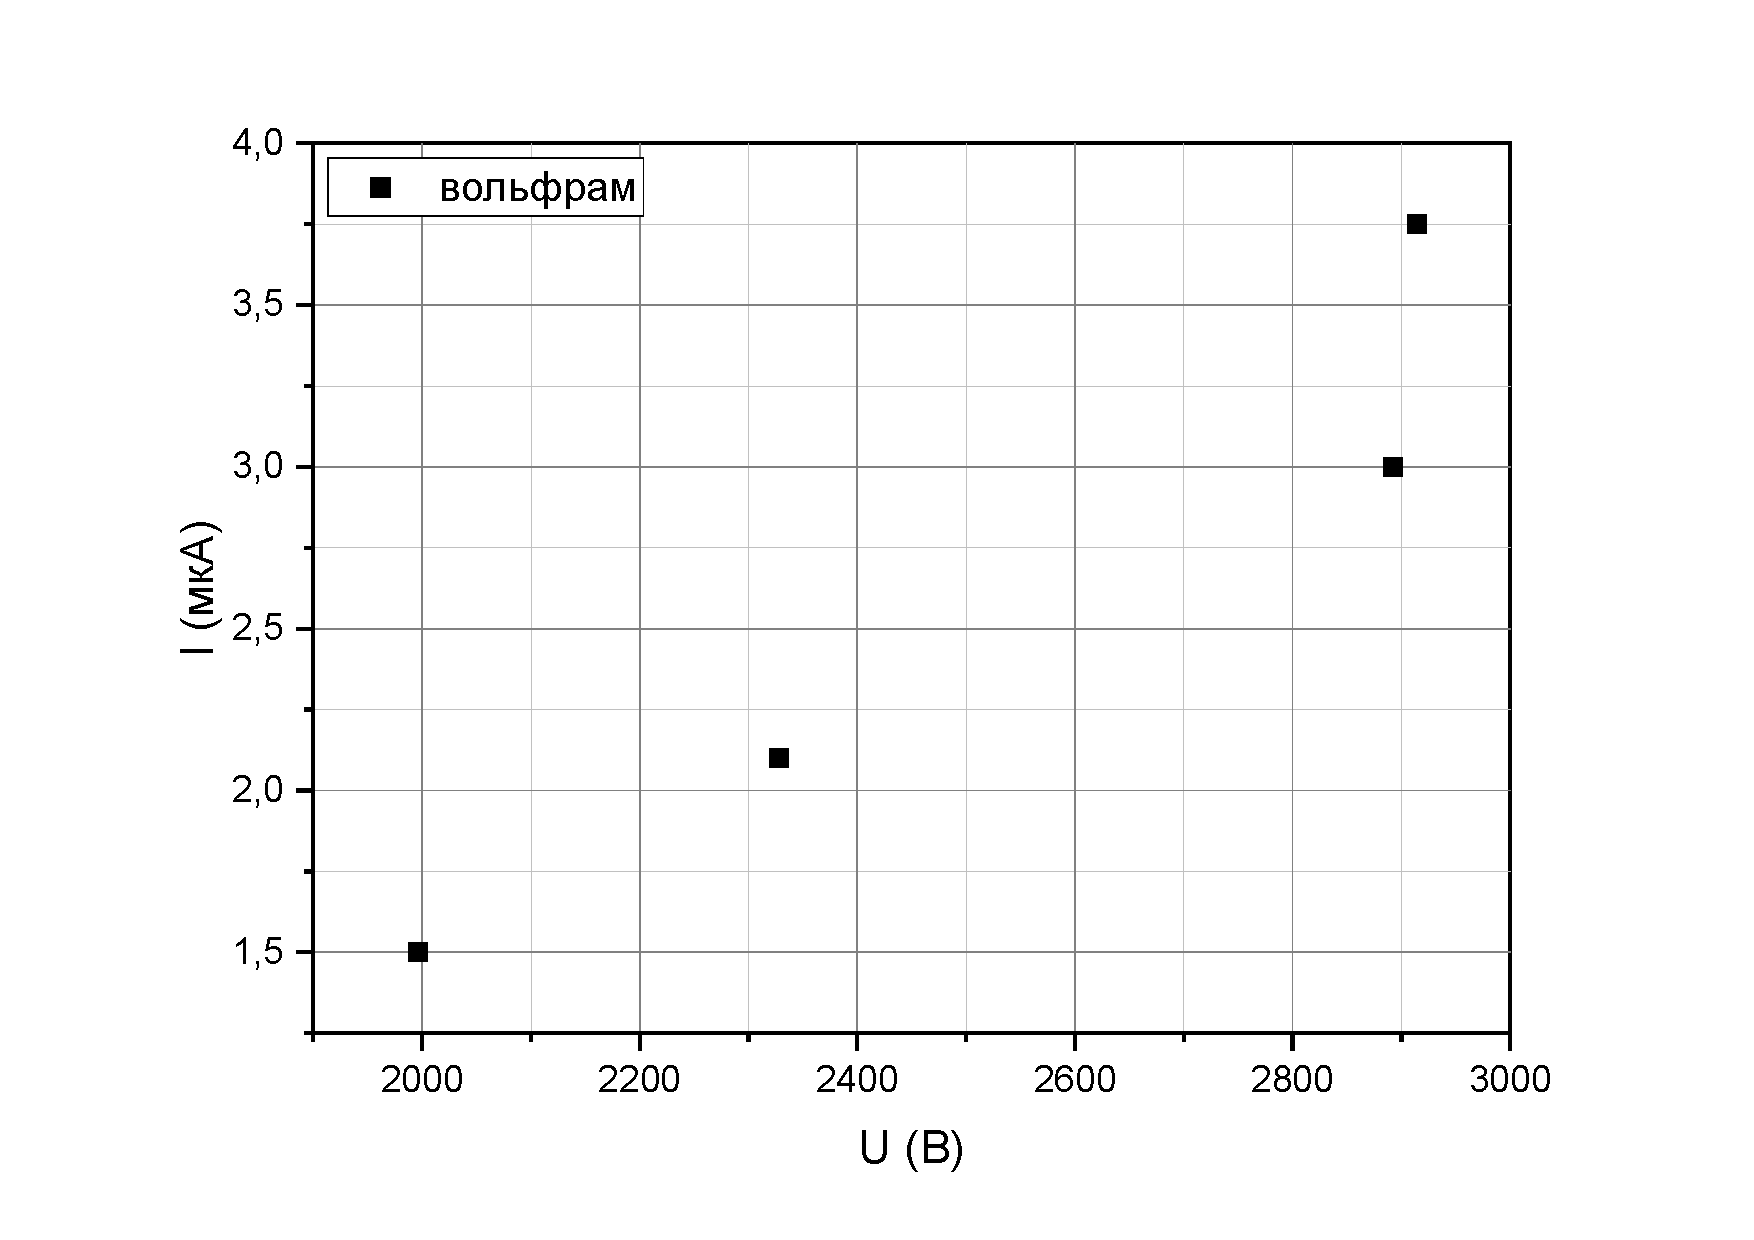
\includegraphics[width=0.65\linewidth]{vakh_volfram.pdf}
\end{figure}

В ходе эксперимента не удалось снять экспериментальные данные для вольфрамовой иглы, так как установка не поддерживала ток. Полученные экспериментальные данные не позволяют дать никакой аналитической оценки зависимости.


\subsection{Исследование автоэмиссионных свойств углеродных материалов}

Снимем вольт-амперную характеристику углеродных трубок. На основании полученных данных построим график зависимости $I = f(U)$.\\
\textbf{Таблица 2. }Данные для построения вольт-амперной характеристики углеродных трубок
\begin{table}[]
\begin{tabular}{|l|l|l|l|l|l|llllllll}
\hline
$I$, мкА & 3    & 5    & 8,25 & 15   & 21   & \multicolumn{1}{l|}{25,5} & \multicolumn{1}{l|}{30}  & \multicolumn{1}{l|}{35}  & \multicolumn{1}{l|}{45}  & \multicolumn{1}{l|}{51}  & \multicolumn{1}{l|}{55}  & \multicolumn{1}{l|}{62}  & \multicolumn{1}{l|}{69}  \\ \hline
$U$, В   & 580  & 640  & 690  & 766  & 813  & \multicolumn{1}{l|}{844}  & \multicolumn{1}{l|}{856} & \multicolumn{1}{l|}{901} & \multicolumn{1}{l|}{935} & \multicolumn{1}{l|}{950} & \multicolumn{1}{l|}{958} & \multicolumn{1}{l|}{979} & \multicolumn{1}{l|}{993} \\ \hline
$I$, мкА & 75   & 80   & 87,5 & 93,5 & 97,5 &                           &                          &                          &                          &                          &                          &                          &                          \\ \cline{1-6}
$U$, В   & 1004 & 1018 & 1037 & 1051 & 1062 &                           &                          &                          &                          &                          &                          &                          &                          \\ \cline{1-6}
\end{tabular}
\end{table}
\begin{figure}[H]
\centering
	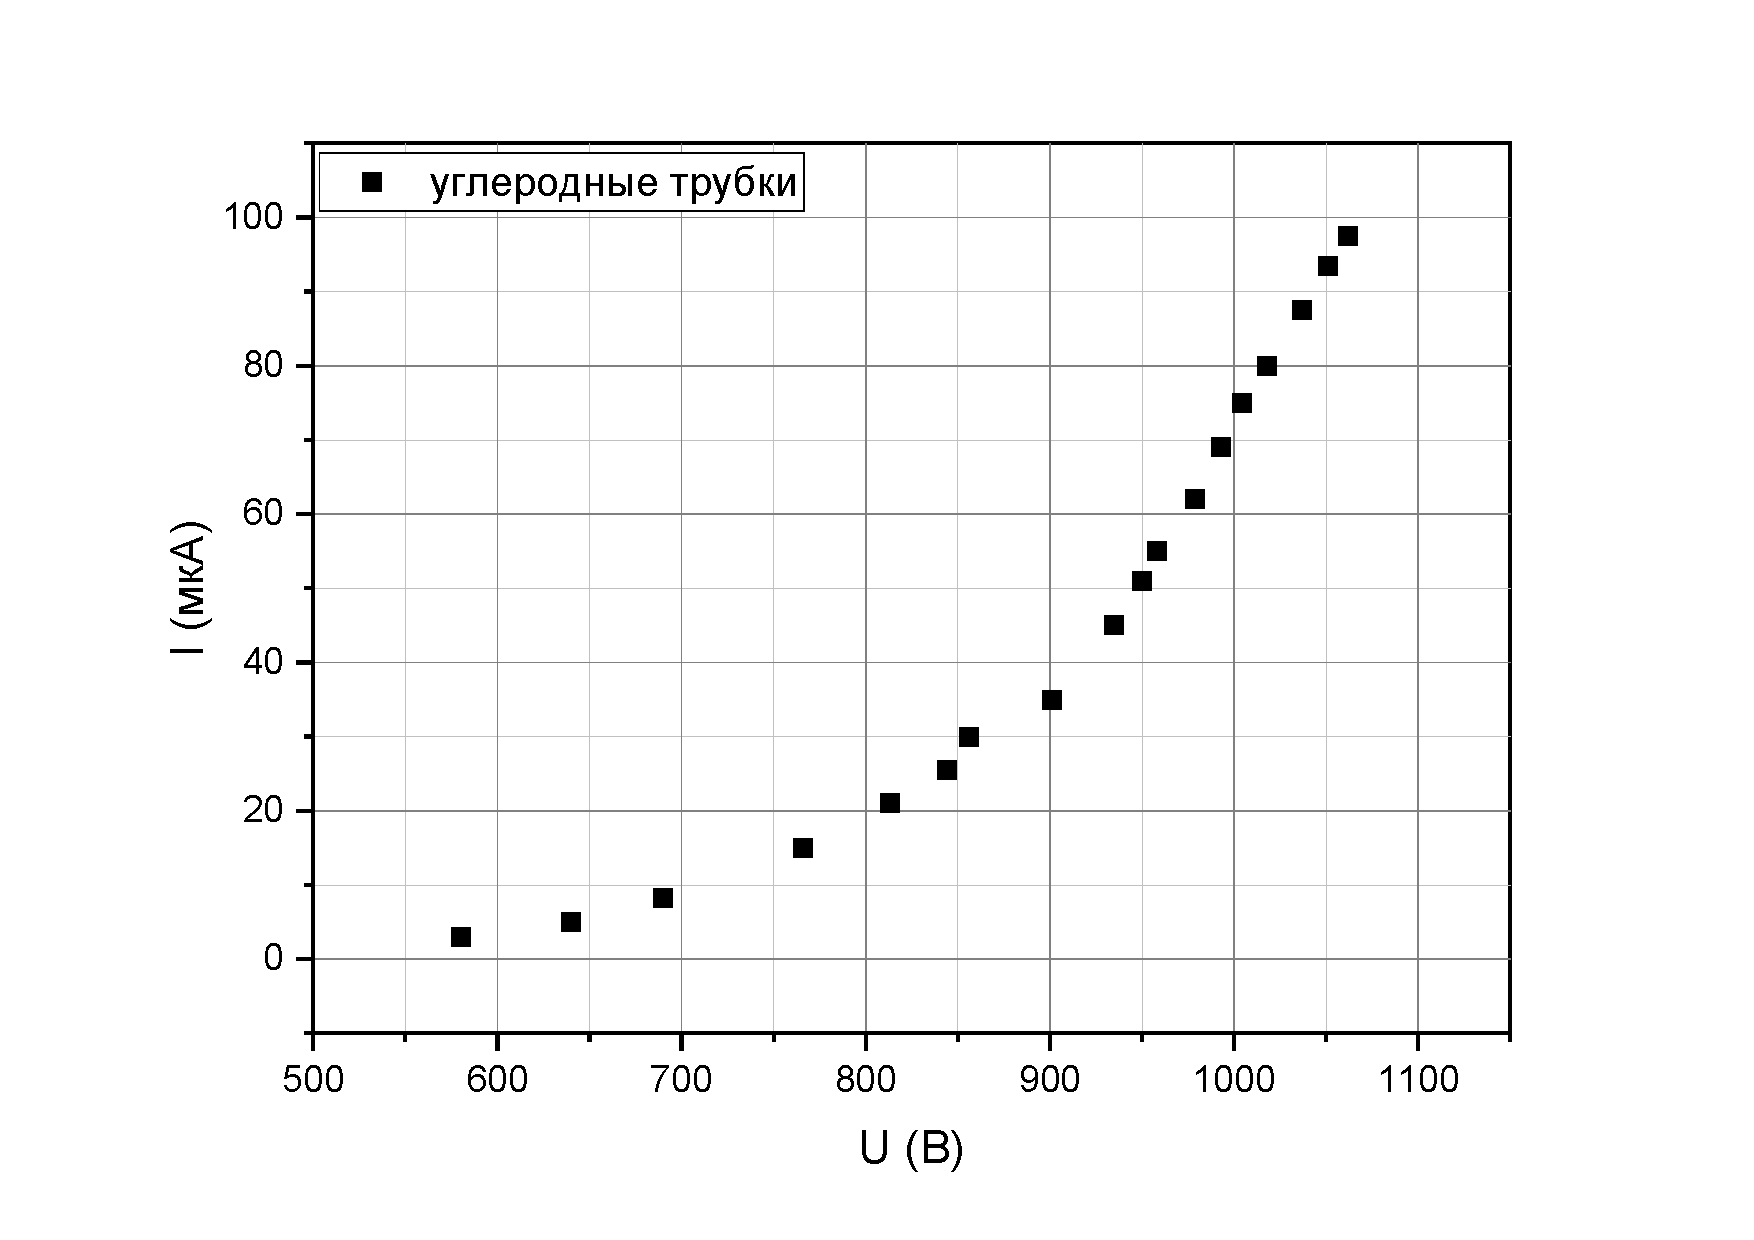
\includegraphics[width=0.65\linewidth]{vakh_uglerod.pdf}
\end{figure}

Построим вольт-амперную характеристику катода в координатах Фаулера - Нордгейма $\ln(I/U^2) = f(1/U)$. 

\begin{figure}[H]
\centering
	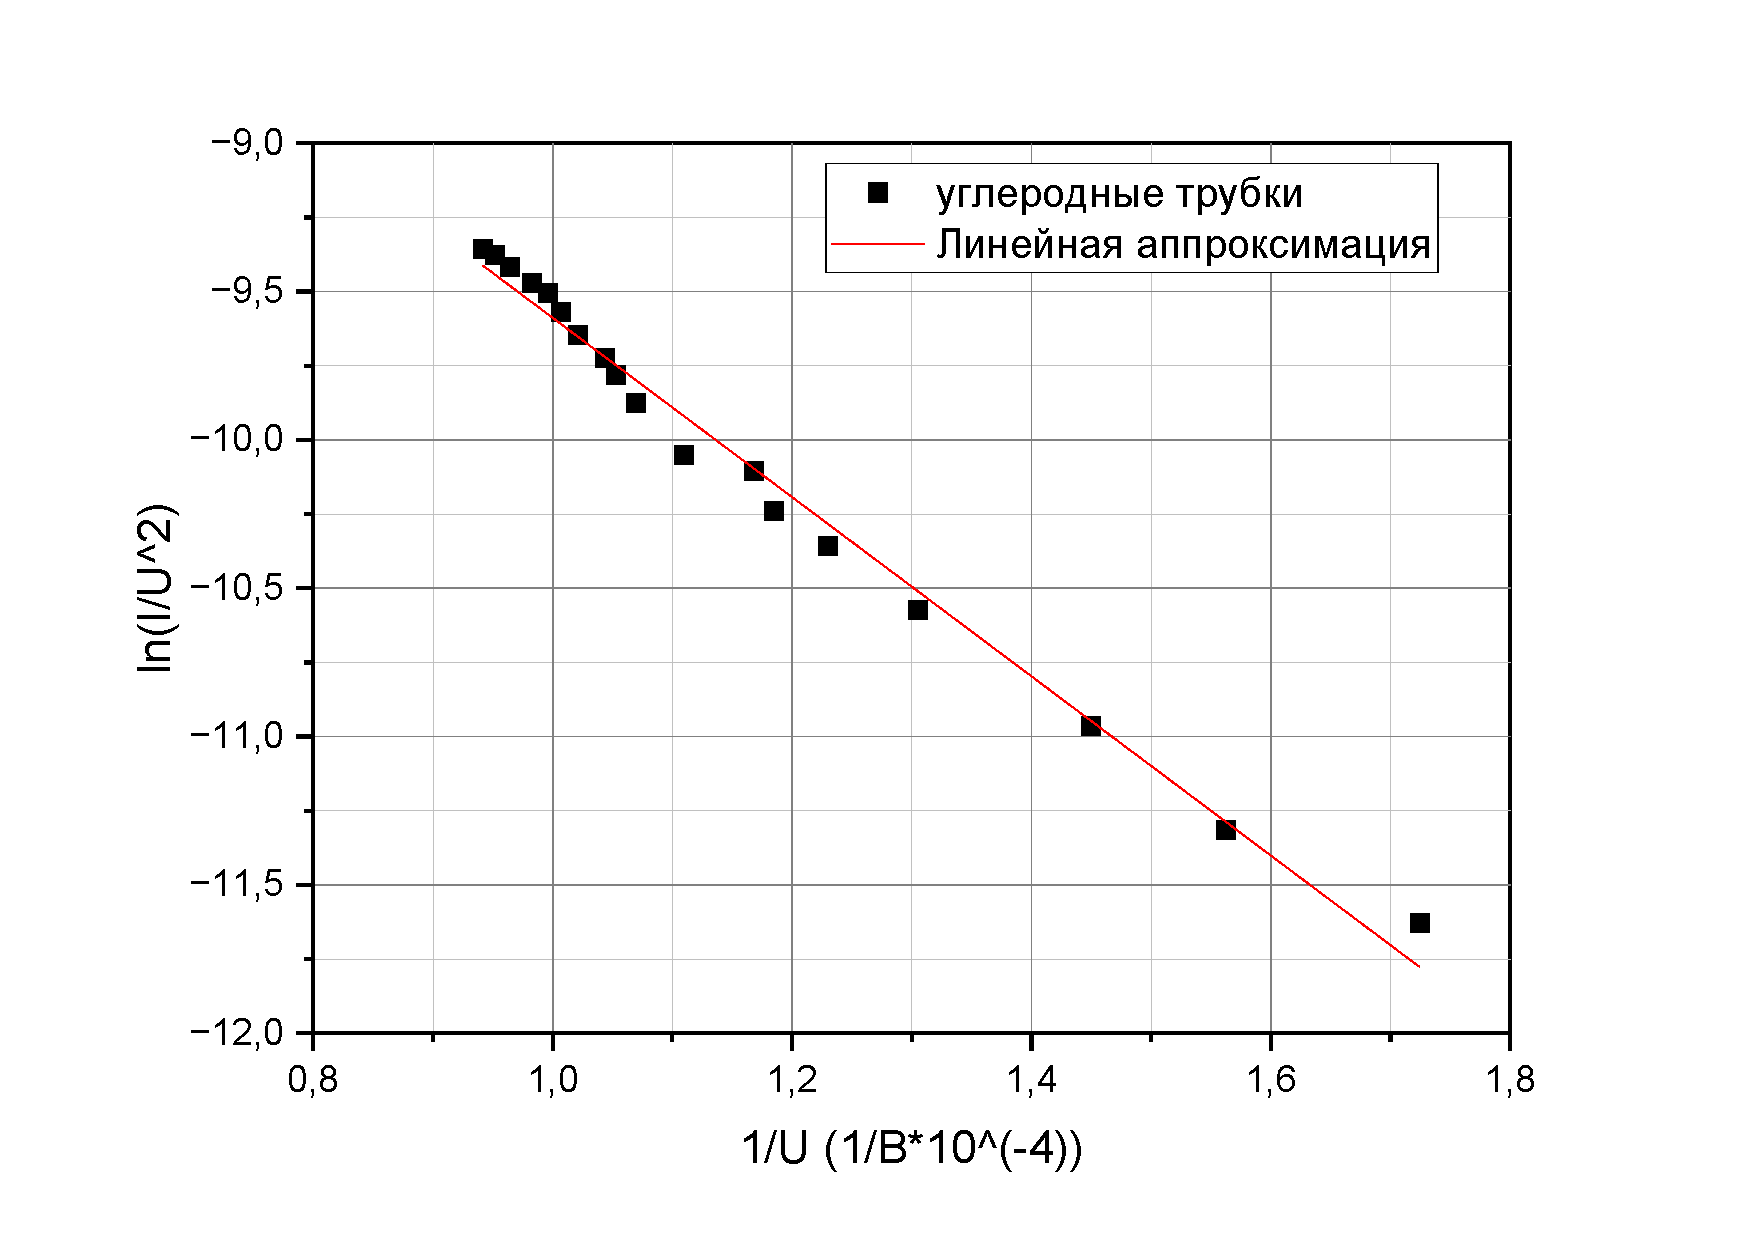
\includegraphics[width=0.65\linewidth]{uglerod.pdf}
\end{figure}

Видим, что график аппроксимируется прямой $y = kx +b$, где $k = -3,02 \pm 0,08$, $b = -6,57 \pm 0,09$. 

По полученным данным можно заметить, что зависимость смещения кривой $b$ от логарифма коэффициента наклона $\ln(k)$ принимает вид прямой. Тогда можно предположить, что флуктуация тока определяется изменением работы выхода, то есть имеет место адсорбция и десорбция атомов остаточных газов. 


\subsection{Получение ВАХ с помощью электронного осциллографа}
Чтобы получить ВАХ при увеличении напряжения с нуля, мы подсоединяем к системе резистор с сопротивлением 26.86 кОм. Мы выбрали резистор с большим сопротивлением, так как в этом случае мы увеличим точность наших измерений и увеличим значение напряжения на данном резисторе. После подключения генератора к каналу 1 (желтая линия) и резистор к каналу 3 (синия линия), снимаем их зависимость от времени.\\\\
\begin{flofigure}
    \centering
    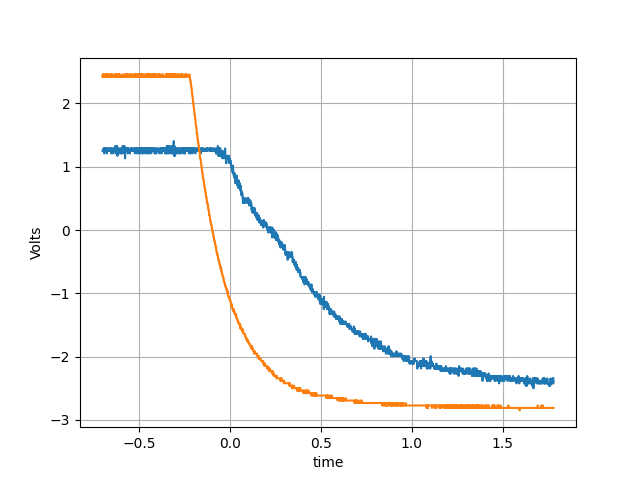
\includegraphics[width=9.5cm]{Oscillograph(time).png}
    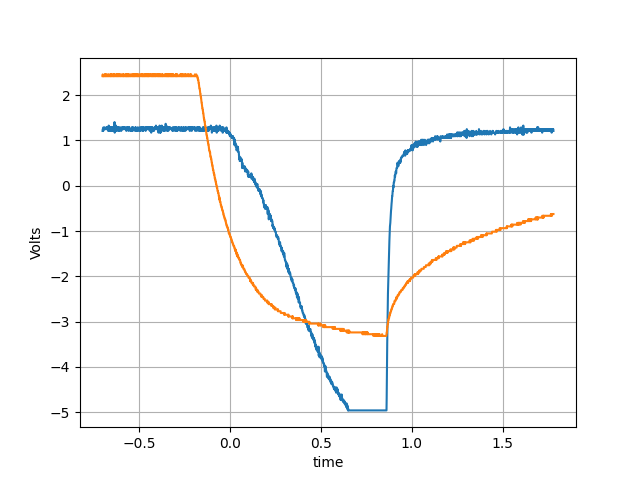
\includegraphics[width=9.5cm]{Proboi(time).png}
    \label{fig:my_label}
\end{flofigure}\\\\
Повторяем данное измерение несколько раз, однако форма кривых практически не изменяется, поэтому не будем рассматривать каждый случай. Учитывая смещения и масштаб графиков построим ВАХ для обоих случаев:\\\\
\begin{flofigure}
    \centering
    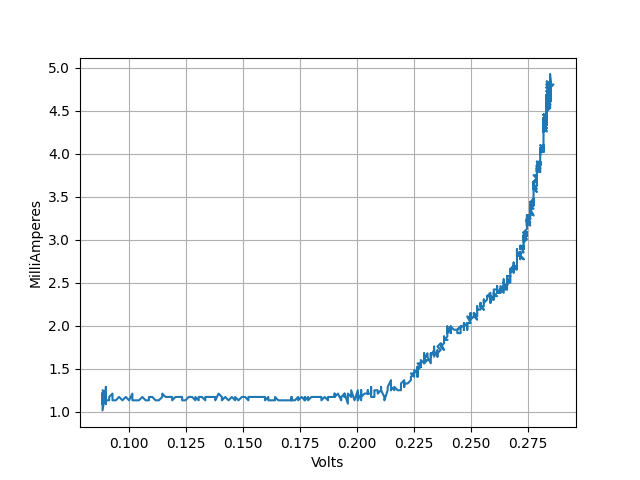
\includegraphics[width=9.5cm]{ВАХ(обычный).png}
    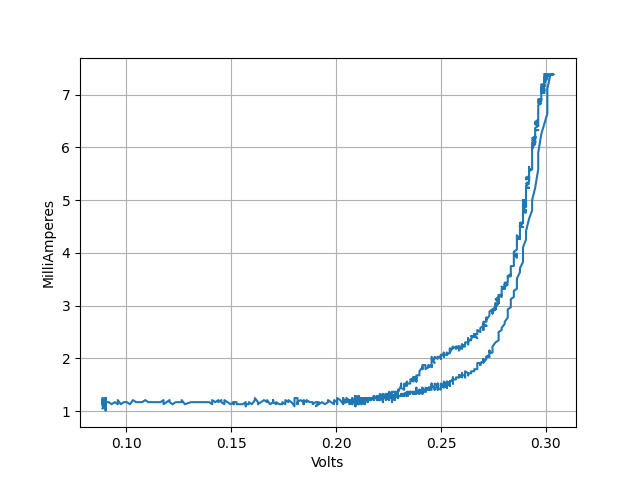
\includegraphics[width=9.5cm]{ВАХ(пробой).png}
    \label{fig:my_label}
\end{flofigure}\\

Заметим, что зависимость не становится линейной в координатах Фаулера - Нордгейма. Это подтверждает предположение, что в установке вольфрамовый катод работает неправильным образом.

\section{Выводы}

В данной лабораторной работе мы изучили особенности автоэлектронной эмиссии и её применения. Исследовали автоэмиссионные свойства вольфрамового острия и катодов, изготовленных из углеродных волокон. Построили вольтамперные характеристики. Как и ожидалось, зависимость в координатах Фаулера - Нордгейма описывается прямой, что подтверждает теорию. Исследовали механизмы нестабильности автоэмиссионного тока на примере углеродных трубок, в нашем случае получили, что имеет место адсорбция и десорбция остаточных газов. 
Также получили ВАХ с помощью электронного осциллографа.

\end{document}
